%Cap4b 7
\begin{frame}{Ascensión de colinas continuación}
Es útil considerar el paisaje del espacio de estados imagen \newline
    \begin{figure}[t]
        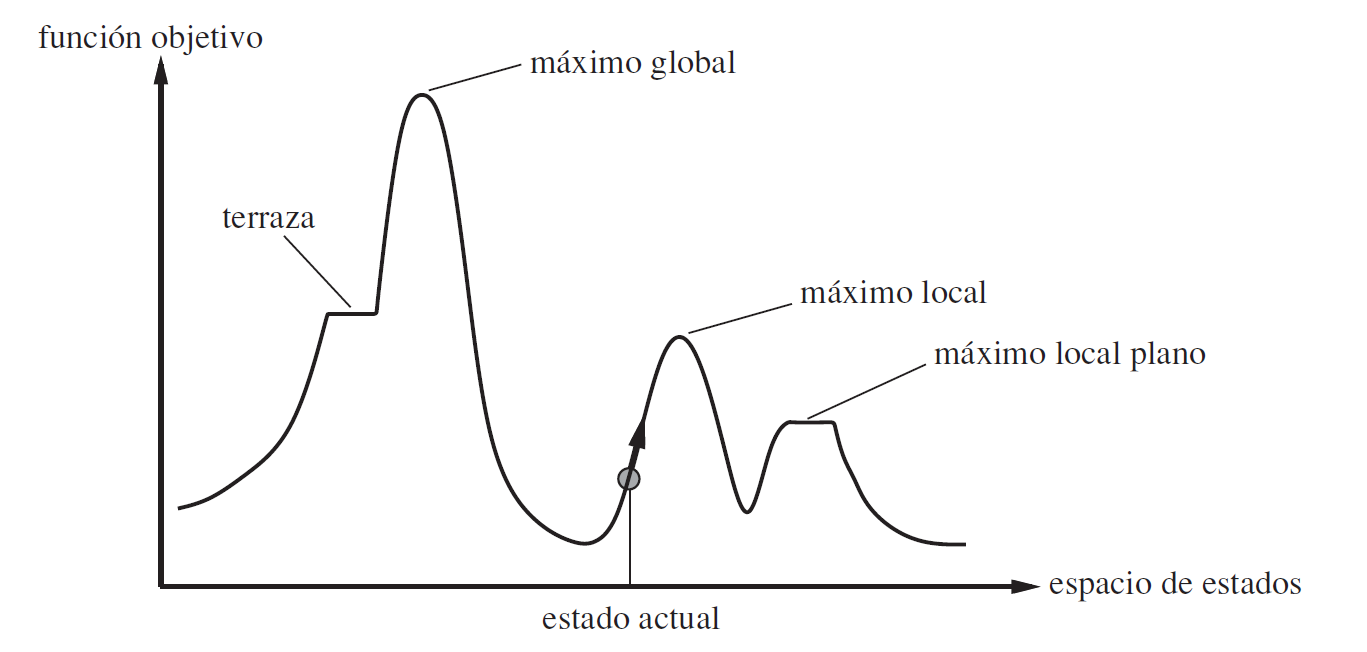
\includegraphics[scale = 0.2]{4b_function.png}
    \end{figure}
\textcolor{blue}{Ascensión de colinas con inicio aleatorio} supera el máximo local - se completatrivialmente \newline
\textcolor{blue}{Movimientos aleatorios a lo lados} \Frowny{} escapa de la terraza  \Smiley{} bucle en máximo local plano
\end{frame}
